\subsection{Methods}
The encoded space of a classical Autoencoder can be very irregular, and small perturbations can lead to very big changes, as we will see in Section \ref{sec:enc}.
To eliminate this problem a new type of Autoencoder has been introduced, called Variational Autoencoder. We so make the mapping probabilistic: the encoder now gives as output a
vector of means $\vec{\mu}$ and the covariances $\vec{\sigma}$ of the input distribution over the encoded space. 
To reduce the complexity we do not generate a $N\times N$ covariance matrix, but simply assume that it is diagonal, using only a vector.
We then regularize the loss function $l$ such that the resulting distribution is 
as close as possible to a multivariate gaussian using the Kulba-Leiber divergence. Calling $x$ the original sample and $\hat{x}$ the reconstructed one:
$$
l = MSE(x, \hat{x})+\lambda KL(\mathcal{N}(\vec{\mu}, \vec{\sigma}), \mathcal{N}(\vec{0}, \vec{1})) = 
MSE(x, \hat{x}) +\frac{\lambda}{2}\sum_{i=1}^N \left( \sigma_i^2+\mu_i^2-1-\ln(\sigma_i^2) \right)
$$
where with $MSE$ we denote the mean square error and $\lambda$ a parameter to control the importance of the "gaussian regularization". 

There is however a problem: the sampling is a discrete process, along which we cannot backpropagate. We so introduce a trick that 
mimicks the sampling, i.e. if we have $\vec{z}\sim \mathcal{N}(\vec{\mu}, \vec{\sigma})$ we can write:
\begin{equation}
    \vec{z} \simeq \vec{\mu} + \vec{\zeta} \vec{\sigma} \quad \mbox{ with } \vec{\zeta} \sim \mathcal{N}(\vec{0}, \vec{1})
\end{equation}
We can now apply the backpropagation.

\subsection{Results}
The variational autoencoder seems to perform well. It was particularly important to tune the parameter $\lambda$, since it strongly affected
the results. A too high $\lambda$ simply resulted in a blurred image for every input, while a too low $\lambda$ produced the same results as the 
classical autoencoder (as expected). We finally fixed it at $\lambda=10^{-5}$.
However, the variational autoencoder works correctly, with a test loss of $0.05$. The encoded space seemed more regular, as we can observe in Figure
\ref{fig:smooth}, where we kept fixed all the components of the encoded samples but one.

\begin{figure}[h]
    \centering
    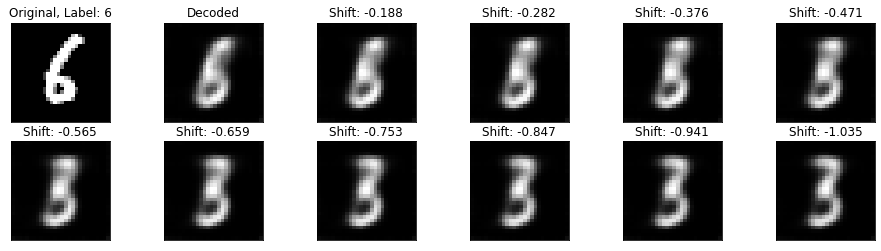
\includegraphics[width=0.8\textwidth]{Images/shift6-3.png}
    \caption{Smooth evolution of the digit $6$ by varying the $0$-th component of its encoded representation by $1/5$ of its original value in each 
        of the figures. The images should be read from left to right, starting from the top row. We notice that the digit changes smoothly from $6$
        to $3$.}
    \label{fig:smooth}
\end{figure}